\chapter{Language Modelling: Foundations, Scale, and Efficiency}

This chapter provides an overview of concepts and terminology used throughout this thesis. I begin by defining the language modelling task and discussing key concepts such as word embeddings and the Transformer architecture. I then discuss how language models are trained and evaluated, including methods to train models more efficiently. The final section motivates a human-centred approach to language modelling and introduces curriculum learning and syntactic generalisation as cognitively inspired frameworks that guide the empirical work in subsequent chapters. Key terms and frequently referenced resources are \thesishl{highlighted} throughout.

\section{How to Model Language}
\label{sec:lm-foundations}

\thesishl{Language modelling} refers to the task of assigning probabilities to sequences of words or tokens. The goal is to model the likelihood of a sequence in a language. In the case of a sequence of words, $w = w_1, w_2, \ldots, w_n$, the probability of the sequence is given by the product of the probabilities of the words occurring in the sequence:

\begin{equation}    
    P(w) = P(w_1, w_2, \ldots, w_n) = \prod_{i=1}^n P(w_i | w_1, \ldots, w_{i-1})
\label{eq:lm-joint-distribution}
\end{equation}

Training a language model is then equivalent to finding a set of parameters that maximise the likelihood of observing the training data; for this reason, language modelling is typically framed as a \thesishl{maximum likelihood estimation} problem. The earliest language models were based on n-gram statistics \citep{jelinek1975design, shannon1948mathematical}, where the probability of a word depends only on the preceding $n-1$ words. While simple and effective, these models suffer from data sparsity and limited context, motivating the development of neural approaches.

\subsection{Neural Language Models}
\label{sec:neural-language-models}

A major breakthrough came with the introduction of neural probabilistic language models by \cite{bengio2003neural}, which proposed using \thesishl{feed-forward neural networks (FFNs)} to estimate the probability of word sequences. In this formulation, the model takes as input a fixed-size context of preceding words, represented as dense vectors (see \cref{sec:word-embeddings}), and passes them through one or more fully connected layers with nonlinear activations (see activation functions in \cref{sec:optimization}). Formally, given a vectorised representation of a concatenated sequence of words $\mathbf{x} = [\mathbf{x}_1; \dots; \mathbf{x}_n]$, where each word, $w_i$, is represented as a vector $\mathbf{x}_i$, the input is processed by a feed-forward neural network as:
\begin{equation}
\mathbf{h} = \phi(W_1 \mathbf{x} + \mathbf{b}_1),
\end{equation}
\begin{equation}
\mathbf{y} = \text{softmax}(W_2 \mathbf{h} + \mathbf{b}_2),
\end{equation}
where $W_1$, $W_2$, $\mathbf{b}_1$, and $\mathbf{b}_2$ are learned parameters, $\phi$ is a non-linear function (see \cref{sec:optimization}), softmax is defined as $\text{softmax}(x)_i = \frac{\exp(x_i)}{\sum_{j=1}^n \exp(x_j)}$ and $\mathbf{y}$ is the predicted probability distribution over the vocabulary for the next word.

\label{sec:word-embeddings}
\label{sec:tokens-vs-words}
Early neural language models introduced \thesishl{word embeddings}: dense vector representations that capture syntactic and semantic relationships between words \citep{mikolov2013efficient, pennington2014glove}. These embeddings enabled \thesishl{transfer learning} in NLP, where pre-trained representations are reused for downstream tasks. In practice, modern language models operate not on whole words but on \thesishl{tokens} that are subword units produced by a tokenisation method like \thesishl{Byte Pair Encoding (BPE)} \citep{sennrich2016bpe}; I use "tokens" throughout this thesis to refer to whatever atomic units a model processes. One of the key problems with early embedding methods was that they were static, assigning the same vector to a token regardless of context. 

% Traditional word embeddings, however, are static, assigning the same vector to a token regardless of context. 


% However, traditional word embeddings are static, assigning the same vector to a word regardless of context. In practice, modern language models operate not on whole words but on sub-word \thesishl{tokens}. To produce these a tokeniser is used to split the text into these smaller atom units; a popular choice for tokenisation is \thesishl{Byte Pair Encoding (BPE)} \citep{sennrich2016bpe} which I use throughout experiments in this thesis. 


% these are atomic units of text that are produced by a tokeniser, such as \thesishl{Byte Pair Encoding (BPE)} \citep{sennrich2016bpe}.

% Moreover, while words are natural linguistic units, modern language models process \thesishl{tokens} with semantic meaning. Modern approaches use \thesishl{Byte Pair Encoding (BPE)} \citep{sennrich2016bpe} to split text into \thesishl{subwords}. The \thesishl{vocabulary size} determines how many tokens the model can use; throughout this thesis, I use ``tokens" to refer to these atomic processing units.

\subsection{Contextualisation and Attention}
To address the limitations of static embeddings, \thesishl{attention mechanisms} were introduced, initially to solve the sequence alignment problem in machine translation \citep{bahdanau2015neural,luong2015effective}. Attention allows models to dynamically focus on the most relevant parts of the input sequence when producing each output token. More formally, given a learned \thesishl{query vector} $\mathbf{q}$ for the current word, and sets of learned \thesishl{key vectors} $[\mathbf{k}_0, \ldots, \mathbf{k}_n]$ and \thesishl{value vectors} $[\mathbf{v}_0, \ldots, \mathbf{v}_n]$ for the other words in the sequence, the attention mechanism computes a weighted sum of the values:
\begin{equation}
\text{Attention}(\mathbf{q}, K, V) = \sum_{i=1}^{n} \alpha_i \mathbf{v}_i,
\end{equation}
where the attention weights $\alpha_i$ are computed using a compatibility function, typically the \thesishl{scaled dot-product}:
\begin{equation}
\alpha_i = \frac{\exp\left(\frac{\mathbf{q} \cdot \mathbf{k}i}{\sqrt{d_k}}\right)}{\sum_{j=1}^{n} \exp\left(\frac{\mathbf{q} \cdot \mathbf{k}_j}{\sqrt{d_k}}\right)},
\end{equation}
with $d_k$ denoting the dimensionality of the key vectors. 

These contextualisation approaches paved the way for the attention-based Transformer architecture.

\subsection{The Transformer}
The introduction of the \thesishl{Transformer} architecture by \citet{vaswani2017attention} marked a turning point in language modelling. The Transformer extends the notion of attention by introducing \thesishl{multi-head attention}, which allows the model to attend to different parts of the sequence from multiple representation subspaces simultaneously. Instead of computing a single attention function, the input is projected into multiple sets of queries, keys, and values:
\begin{equation}
\text{MultiHead}(Q, K, V) = \text{Concat}(\text{head}_1, \dots, \text{head}_h)W^O,
\end{equation}
where each head is computed as:
\begin{equation}
\text{head}_i = \text{Attention}(QW_i^Q, KW_i^K, VW_i^V).
\end{equation}
Here, $W_i^Q, W_i^K, W_i^V$ are parameter matrices for the $i$-th head, and $W^O$ is an output projection matrix that combines the outputs of the individual attention heads. This design allows each head to capture distinct types of relationships between tokens, thereby enriching the final representation.

Most importantly, the Transformer model helped establish the \thesishl{pre-train--fine-tune} paradigm as the standard approach in modern language modelling. Rather than using static embeddings from separate models, Transformer models learn contextualised representations directly from data through \thesishl{pre-training} on \thesishl{self-supervised objectives}; these are training tasks that require no human-labelled data and instead derive supervision from the structure of the text itself. These objectives, such as predicting masked tokens or next tokens in a sequence, either directly optimise the language modelling probability distribution (see \cref{eq:lm-joint-distribution}) or learn representations that indirectly capture the statistical patterns needed for language understanding. The model then adapts these learned representations to specific tasks through \thesishl{fine-tuning}. How these self-supervised objectives are defined is the subject of the next section.



\subsection{Transformer-based Language Models}

Building on the Transformer architecture, \thesishl{BERT}~\citep{devlin2019bert} popularised the \thesishl{masked language modelling (MLM)} objective, where some percentage of input tokens are replaced with a special [MASK] token, and the model is trained to predict the original identity of these masked tokens given their context. Formally, for a sequence of tokens $T = (t_1, \ldots, t_n)$ and a set of masked positions $M \subset \{1, \ldots, n\}$, the MLM objective maximises
\begin{equation}
    \mathcal{L}_{\text{MLM}} = \sum_{i \in M} \log P(t_i \mid t_{\setminus M}),
\end{equation}
where $t_{\setminus M}$ denotes the sequence with masked tokens replaced by [MASK]. This enables BERT to learn deep bidirectional representations, as the model can attend to both left and right context. Note that models trained to maximise the MLM objective do not directly learn a joint-distribution over the entire sequence of words as is typically assumed in language modelling (see \cref{eq:lm-joint-distribution}). Following BERT, \thesishl{RoBERTa}~\citep{liu2019roberta} improved on its design by removing the next sentence prediction task and scaling up training data. RoBERTa serves as the base architecture for experiments in Chapters 3 and 4 of this thesis. %Other notable variants include ALBERT~\citep{lan2019albert}, which introduces parameter sharing, and DistilBERT~\citep{sanh2019distilbert}, which compresses BERT via knowledge distillation.

In contrast to masked language modelling, autoregressive pre-training, as used in the popular \thesishl{GPT} series~\citep{radford2018gpt1, radford2019gpt2, brown2020gpt3}, trains models to predict each token based only on its preceding context. This so-called \thesishl{autoregressive (AR)} objective maximises the likelihood:

\begin{equation}
\mathcal{L}_{\text{AR}} = \sum_{i=1}^n \log P(t_i \mid t_1, \ldots, t_{i-1}),
\label{eq:ar-loss}
\end{equation}

enforcing a unidirectional, left-to-right dependency. Autoregressive models learn a joint probability distribution over the entire sequence, making them `generative' models that can sample text. Today, autoregressive models are the most widely used for text generation tasks.


\subsection{Training and Optimisation}
\label{sec:optimization}

In practice, training language models involves several interconnected components. Central to the training process is the choice of optimisation algorithm. Models are typicaly trained using \thesishl{gradient descent}, which iteratively updates model parameters to minimise a loss function. For a model with parameters $\theta$ and loss function $\mathcal{L}(\theta)$, the update rule at timestep $i+1$ is:
\begin{equation}
    \theta_{i+1} = \theta_i - \alpha \nabla_{\theta_i} \mathcal{L}(\theta_i)
\end{equation}
where $\alpha$ is the \thesishl{learning rate} and $\nabla_{\theta_i} \mathcal{L}(\theta_i)$ is the gradient of the loss. Computing gradients over an entire dataset is usually infeasible, so in practice gradients are estimated over mini-batches via stochastic gradient descent.  Modern training relies on adaptive optimisers such as \thesishl{AdamW} \citep{loshchilov2019decoupled}, which combines momentum (using exponential moving averages of past gradients to smooth updates) with per-parameter adaptive learning rates. The learning rate is typically managed through scheduling (e.g. warm-up followed by decay) and gradient clipping to prevent instability. 

Beyond optimisation, successfully training a language model requires careful architectural decisions. Non-linear \thesishl{activation functions} are essential for enabling neural networks to learn complex mappings. Common choices for modern Transformers include GELU \citep{hendrycks2016gaussian} in encoder models like BERT, and \thesishl{SwiGLU} \citep{shazeer2020glu}, which incorporates a gating mechanism, in decoder-only architectures like GPT.

Regularisation and normalisation techniques also play a critical role in ensuring that the model generalises well to new data. These techniques seek to prevent model \thesishl{overfitting} which occurs when a model memorises training data rather than learning generalisable patterns. Dropout \citep{srivastava2014dropout} does so by randomly deactivating units during training, forcing the network to develop more robust representations. \thesishl{Layer Normalisation} \citep{ba2016layernorm} stabilises training by normalising activations across features within each layer, reducing sensitivity to initialisation and learning rate. Modern Transformers typically apply normalisation before each attention layer, a strategy known as \thesishl{Pre-Layer Normalisation} \citep{xiong2020layer}.

Several additional architectural enhancements have become standard in modern language models. First, in order to explicitly encode the position of tokens in the sequence, position-encoding techniques are used. One popular method is \thesishl{Rotary Position Embeddings (RoPE)} \citep{su2024rope} which encode position through rotation matrices applied to query and key vectors. Secondly, \thesishl{Residual connections} \citep{he2016deep}, which add a layer's input directly to its output, facilitate gradient flow through deep networks and enable training of architectures with hundreds of layers. Finally, \thesishl{Grouped Query Attention (GQA)}~\citep{ainslie2023gqa} reduces memory requirements during inference by having multiple query heads share a single set of key and value projections. These components are all used in the \pico framework (Chapter 7).

\subsection{Datasets and Evaluation}
The performance of language models depends critically on the scale, diversity, and quality of their pre-training data. Two datasets are particularly relevant to this thesis. \thesishl{The Pile} \citep{gao2020pile} is a 250-billion-token curated corpus assembled from 22 diverse sources, including academic papers, books, code repositories, and web text; it was used to train the \thesishl{Pythia} model suite \citep{biderman2023pythia}, which I analyse in Chapter 6. \thesishl{Dolma} \citep{soldaini2024dolma} is a more recent 3-trillion-token dataset designed for reproducible research, combining web crawls, scientific literature, and curated sources; I use it to train the \pico model suite in Chapter 7.

Evaluating language models can be done using both intrinsic metrics that measure how well a model captures language statistics and extrinsic benchmarks that test downstream task performance. \thesishl{Perplexity} \citep{jelinek1977perplexity} is a standard intrinsic metric, computed as the exponentiated average negative log-likelihood over a held-out corpus (see \cref{eq:ar-loss}). For extrinsic evaluation, several benchmark suites are used throughout this thesis. The General Language Understanding Evaluation (\thesishl{GLUE}) benchmark \citep{wang2018glue} comprises a collection of natural language understanding tasks, including sentiment analysis (SST-2), linguistic acceptability judgments (CoLA), and natural language inference (MNLI, QNLI), and is used for evaluation in Chapter 4. \thesishl{SuperGLUE} \citep{wang2019superglue} was introduced as a more challenging successor, featuring tasks that require more sophisticated reasoning, and is used in Chapter 3. \thesishl{HellaSwag}~\citep{zellers2019hellaswag} tests commonsense reasoning by asking models to select the most plausible continuation of a scenario, and is used to evaluate models in Chapter 7. Finally, linguistically-targeted benchmarks such as the Benchmark of Linguistic Minimal Pairs (\thesishl{BLiMP}) and MSGS \citep{warstadt2020blimp, warstadt2020msgs} use carefully constructed minimal pairs (i.e., sentences differing in only one critical aspect) to probe whether models have acquired specific grammatical knowledge.

\subsection{Strategies for Efficient Training}
Training language models is computationally expensive and motivates the development of more efficient training strategies. Here I list just a few of the most common strategies.

\thesishl{Knowledge distillation} trains a compact "student" model to replicate the behaviour of a larger "teacher" model, typically by matching the teacher's output probability distributions rather than just the hard labels \citep{hinton2015distilling}. This transfers the teacher's learned representations into a smaller architecture that is cheaper to deploy. DistilBERT~\citep{sanh2019distilbert} demonstrated that this approach can retain over 95\% of BERT's performance with roughly half the parameters and significantly faster inference.

\thesishl{Pruning} reduces model size by identifying and removing weights that contribute little to performance. The \thesishl{Lottery Ticket Hypothesis} \citep{frankle2019lottery} provided theoretical grounding for this approach, showing that large networks contain sparse subnetworks that can match the accuracy of the full model. Pruning methods typically use model statistics and heuristics to decide which weights to prune \citep{lecun1990optimal, hassibi1993optimal,han2016deep}.

\thesishl{Architectural modifications} can also yield substantial efficiency gains. Parameter sharing, as used in ALBERT \citep{lan2019albert}, reduces memory footprint by reusing weights across layers. \thesishl{FlashAttention} \citep{dao2022flashattention} addresses the computational bottleneck of self-attention by restructuring the computation to better exploit GPU memory and results in significant speedups without loss of accuracy.

\thesishl{Parameter-efficient fine-tuning} (PEFT) methods reduce the cost of adapting pre-trained models to new tasks. \thesishl{LoRA} \citep{hu2021lora} freezes the original model weights and injects small, low-rank trainable matrices into attention layers, dramatically reducing the number of parameters that must be updated. \thesishl{ReLoRA} \citep{lialin2023relora} extends this idea to pre-training itself, periodically merging low-rank updates into the base weights and reinitialising the low-rank components. This approach is explored as a case study in Chapter 7.

Finally, recent research challenges the long-standing assumption that massive datasets are necessary for effective language modelling. A growing body of work shows that carefully calibrated training data can enable small models to perform surprisingly well, especially when the input is tailored to the specific competencies desired in a model. In this context, the \thesishl{BabyLM Challenge}~\citep{warstadt2023babylm1, conll2024babylm2} tests the limits of language model training under data-constrained settings that mirror how infants are exposed to language. The challenge requires training on only 10 million words of `cognitively-plausible' data, including child-directed speech from CHILDES~\citep{macwhinney2000childes}, children's literature, and simplified Wikipedia. This challenge serves as the testbed for the experiments in Chapters 3 and 4.

\section{Human-Centered Language Modelling}

\begin{figure}[ht!]
    \centering
    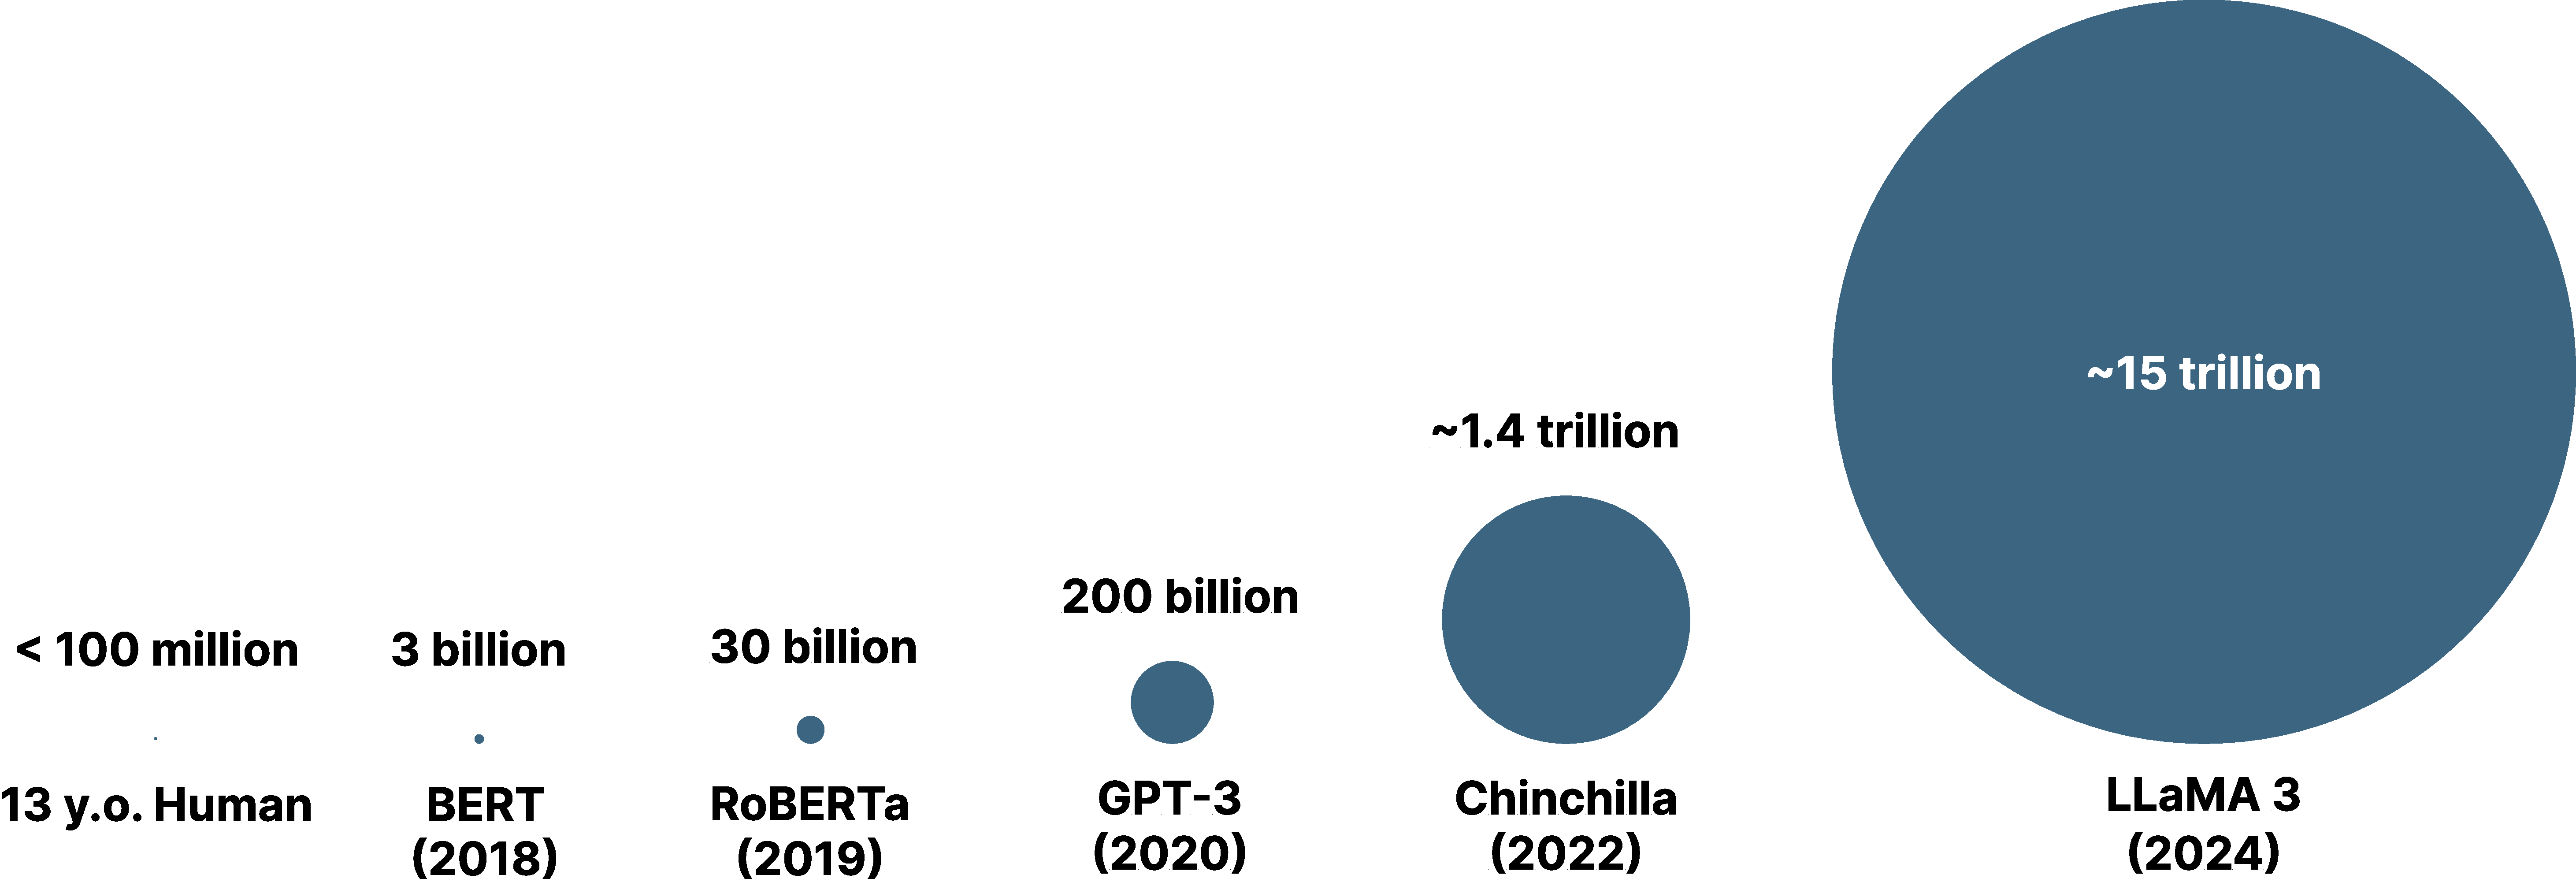
\includegraphics[width=0.7\textwidth]{chapters/background/figures/data_comparison.pdf}
    \caption{Comparison of data scales used by different language modelling approaches. Humans are estimated to observe less than 100 million words by the age of 13.}
    \label{fig:data-comparison}
\end{figure}

While current research directions for improving small model efficiency largely centre on optimisation and architectural innovations, these efforts are generally exploratory; they lack an underlying thesis for how to train models more efficiently. To make more grounded and robust progress in developing efficient training paradigms, it is valuable to establish a guiding framework or set of principles. One promising approach is to draw inspiration from how humans learn. The brain is a biologically constrained system that achieves remarkable linguistic competence with limited resources. \cref{fig:data-comparison} visualises the order of magnitude difference that language models are trained on versus the amount of data humans perceive. In this thesis, I argue that human language acquisition can serve as a framework to inform more efficient model training. In the following chapters, I explore two approaches to language modelling that are inspired by human language acquisition: curriculum learning and syntactic generalisation.


\subsection{Curriculum Learning}

\thesishl{Curriculum learning} draws inspiration from how children acquire language progressively rather than all at once. As \citet{bengio2009curriculum} formalised, this approach involves structuring training to begin with easier inputs and gradually increase complexity over time, rather than exposing models to randomly shuffled data of uniform difficulty. Complexity in the training of a language model can arise across several dimensions:

%This paradigm also maps naturally onto human language production: children do not produce all linguistic phenomena simultaneously, but instead progress from babbling to simple utterances, and eventually to complex syntax and abstract meaning. The BabyLM Challenge \citep{warstadt2023babylm1} provides an ideal testbed for exploring these ideas under cognitively plausible constraints.

% A key challenge in curriculum learning is how to define what makes a training example “easy” or “hard” for a given language model? Learning difficulty can arise from multiple facets of the training setup. For instance, difficulty can be defined via linguistic features of the training data (e.g. sentence length, syntactic complexity, or vocabulary frequency), via model-based metrics (such as computing perplexity or an auxiliary model's loss on a given set of data), or even via human-annotated scores (for example, readability or “surprisal”) \citep{soviany2022curriculum}. Moreover, curriculum learning can be applied to aspects of the training pipeline other than the data. These include:   %In practice, researchers often combine these signals (or use a dynamic curriculum that re-evaluates difficulty periodically) to keep training material in the “zone of proximal development” (or “Goldilocks” zone); that is, neither too easy (so that the model is not challenged) nor too hard (so that learning is not stalled). Current research has explored several dimensions of curriculum learning in NLP.

\paragraph{Progressive vocabulary exposure} A first axis to apply curriculum learning to is the vocabulary of a language model. Studies show children begin with a limited lexicon that expands gradually (by 8-10 words per day) \citep{fenson1994variability, bergelson2015early, weizman2001lexical}, focusing first on concrete nouns and verbs. In contrast, language models traditionally start with a complete vocabulary. Recent work has begun exploring frequency-based vocabulary scaffolding \citep{soviany2022curriculum} so that models gradually acquire a larger vocabulary, akin to human language learners. 

\paragraph{Dynamic data sampling} The most common variant of curriculum learning defines training complexity as the `difficulty' of the training examples shown to a model. A key challenge in this framing is how to define what makes a training example “easy” or “hard” for a given language model. For instance, difficulty can be defined via linguistic features of the training data (e.g. sentence length, syntactic complexity, or vocabulary frequency) \citep{campos2021curriculum, kocmi2017curriculum, liu2018curriculum}, via model-based metrics (such as computing perplexity or an auxiliary model's loss on a given set of data) \citep{sachan2016easy, lalor2020dynamic}, or even via human-annotated scores (for example, readability or “surprisal”) \citep{soviany2022curriculum}. 

\paragraph{Graduated learning objectives} Curriculum learning can also be applied at the level of the objective function used to train a language model. Standard language modelling objectives (such as MLM) that require identifying a masked token as one of possibly thousands of vocabulary items can be quite challenging from the outset. Some approaches have explored beginning with simpler prediction tasks before tackling more complex ones, similar to how children grasp broad categories before mastering precise lexical distinctions \citep{markman1990constraints}. These simpler tasks might involve predicting broad linguistic categories such as hypernyms \citep{bai2022better} or syntactic roles (e.g. predicting part of speech tags) \citep{wang2023language, cui2022lert} rather than specific word identities, thereby reducing the prediction space from thousands of vocabulary items to a smaller set of linguistic categories. These ideas are also inspired by psycholinguistic theories that children first learn coarse linguistic categories and later generalise to a full lexicon \citep{alishahi2010computational, gleitman1990structural}.

\vspace{1em}

While these ideas have been explored individually, there remains significant opportunity for developing more integrated approaches. There is currently no unified framework that systematically implements and evaluates these strategies, especially in small-scale language modelling. Such a framework would be particularly valuable for understanding how different curriculum dimensions (i.e. vocabulary progression, data ordering, and learning objectives) interact and whether curriculum learning as a whole is beneficial for model efficiency and generalisation.

\subsection{Syntactic Generalisation}

While curriculum learning provides a framework for structuring the learning process, another key challenge in language modelling is ensuring robust generalisation to novel linguistic structures. This challenge mirrors a fundamental aspect of human language acquisition: the ability to understand and produce grammatical constructions that may not have been explicitly observed during learning. From an early age, children demonstrate an impressive capacity to abstract syntactic patterns and apply them productively, even with limited exposure \citep{yang2013poverty, legate2002empirical}. This capacity suggests that humans possess strong inductive biases that enable generalisation from sparse and noisy input.

As an illustrative example, take the sentence, ``After lunch, the kids zambled through the garden, giggling and chasing butterflies.'' Even though `zambled' is a made-up word, we can nonetheless infer its syntactic category (verb), morphological structure (past participle), and approximate meaning based on surrounding cues (e.g. `to run joyfully'): a phenomenon known as ``syntactic bootstrapping" \citep{gleitman1990structural, naigles1990children}. This ability highlights the importance of syntax as a scaffold for lexical learning and supports the hypothesis that grammatical structures provide a backbone for interpreting linguistic input. By contrast, language models struggle to incorporate syntactic cues in a similar way to humans due to two key properties inherent to language modelling:

\paragraph{Frequency Bias} While human learners generalise from structure, language models internalise surface-level frequency statistics due to their maximum likelihood training objectives. This results in a strong bias towards predicting frequent tokens and can obscure the model's true syntactic capabilities \citep{feldman2020does, haviv2023understanding}. Human learners, by comparison, rely on structural cues rather than frequency alone, allowing them to recognise grammatical roles even for novel or rare words \citep{tomasello2003constructing}.

\paragraph{Representation Degeneration} Frequency-driven learning can also lead to representation collapse, where embeddings for rare tokens are poorly differentiated. This degeneration leads to \thesishl{anisotropy} in the representation space of embeddings; a phenomenon where the embeddings of all infrequent words converge into a narrow subspace \citep{ethayarajh2019contextual}. In contrast, human mental lexicons maintain separable, richly structured representations for even infrequent words \citep{murphy2002bigbook}.

\vspace{1em}

Some methodologies have been developed to improve the linguistic generalisation of language models. At the lexical level, the integration of morphological and orthographic information during pre-training has been explored to obtain word embeddings that capture morphological structure \citep{salle2018incorporating, vulic2017morphfitting, cotterel2015morphological, bhatia2016morphological, botha2014compositional}. To improve syntactic generalisation, other work has explored enriching the objective function with auxiliary tasks, such as predicting constituency labels \citep{wang2023language}, hypernyms \citep{bai2022better}, dependency tags \citep{cui2022lert}, and POS tags \citep{diehlmartinez2023climb}. Another type of approach directly incorporates grammatical structure into the model architecture itself: Recurrent Neural Network Grammars \citep{dyer2016rnng} jointly model sentences and their phrase structures using stack-based neural networks, while their Transformer-based successors \citep{sartran2022transformer} implement syntactic composition through specialised attention masks. Some approaches have also shown promising results on rare word performance by constructing token embeddings that consider a word's surface form and surrounding context \citep{schick2019attentive, schick2020rare}. These approaches, however, are largely empirically motivated and do not directly address the fundamental challenge that language models face: the distribution of training data, weighted heavily towards frequent tokens, leads to both \textbf{frequency bias} and \textbf{representation degeneration}, and impedes generalisation to infrequent tokens.

I argue that advancing syntactic generalisation in models, especially those constrained in size or training data, requires more principled integration of linguistic theory and cognitive insight.

% \paragraph{Scaling Limitations} Larger model sizes are often needed to approximate the statistical properties of infrequent words, posing a challenge for efficiency and interpretability. Human learners, however, achieve high generalization with dramatically fewer parameters—suggesting the potential of syntactic cues as a source of inductive bias that supports efficient learning from small data \citep{tomasello2003constructing, clark2020emergence}.

% To address these challenges, recent approaches have drawn inspiration from how children integrate linguistic structure into word learning:

% \paragraph{Linguistic Feature Integration} Echoing how children rely on morphosyntactic cues to infer category and meaning \citep{gleitman1990structural, naigles1990children}, several methods enhance token representations with morphological, syntactic, or lexical-semantic information \citep{salle2018incorporating, vulic2017morphfitting, cui2022lert, diehlmartinez2023climb}. These augmentations allow models to generalize more effectively, especially for underrepresented vocabulary.

% \paragraph{Representation Space Optimization} Techniques that mitigate anisotropy in embedding spaces aim to recover a more human-like separation of meanings. By filtering out dimensions dominated by frequency or noise, these methods promote models to learn syntactic organization \citep{arora2016simple, mu2018all, bis2021too}.

% \paragraph{Objective Calibration} Alternative training objectives and regularization strategies seek to reduce frequency bias by explicitly rewarding syntactic consistency and discouraging overfitting to frequent items \citep{gong2018frage, gao2018representation}. These interventions embed a structural bias into learning, allowing even small models to better generalize from limited input—mirroring the efficiency of human learners.

\subsection*{From Cognitive Theory to Computational Practice}

Integrating principles from human learning into language modelling marks a significant shift in the field of language model development. Rather than focusing solely on architectural innovations or computational efficiency, I emphasise drawing from cognitive and developmental theories to design learning protocols that take inspiration from human language acquisition. This perspective should not be read as an attempt to reproduce the biological mechanisms of human language acquisition, but rather as a pragmatic strategy: since we know an efficient system for language learning exists, it is sensible to borrow and test the aspects we do understand as hypotheses for improving small model training.

This thesis explores two complementary approaches to human-inspired language modelling. In Chapter 3, I introduce Curriculum Learning for Infant-inspired Model Building (\climb), a framework developed for the BabyLM Challenge. \climb explores three cognitively inspired curriculum learning strategies: vocabulary progression, data difficulty ordering, and graduated learning objectives. In Chapter 4, I address a fundamental challenge in language modelling: how to achieve robust syntactic generalisation without relying on increasingly large models. I present \smoothing, a method inspired by how children leverage syntactic knowledge to understand novel vocabulary items. In addition, I develop a metric that quantifies the frequency bias of language models, providing a tool to better assess the balance between memorisation and generalisation.

Together, these chapters evaluate how insights from human language acquisition can inform approaches to language modelling, from the macro-level structure of learning (curriculum design) to the micro-level mechanics of representation (syntactic generalisation).


% \subsection{Curriculum Learning}

% \thesishl{Curriculum learning} draws inspiration from how children acquire language progressively rather than all at once. As \citet{bengio2009curriculum} formalised, this approach involves structuring training to begin with easier inputs and gradually increase complexity over time. Complexity in language model training can arise across several dimensions:
% %
% \textit{Progressive vocabulary exposure:} Studies show children begin with a limited lexicon that expands gradually \citep{fenson1994variability, bergelson2015early}. Recent work has begun exploring frequency-based vocabulary scaffolding \citep{soviany2022curriculum} so that models gradually acquire a larger vocabulary.
% %
% \textit{Dynamic data sampling:} Training complexity can be defined via linguistic features (e.g. sentence length, syntactic complexity) \citep{campos2021curriculum, kocmi2017curriculum}, model-based metrics such as perplexity \citep{sachan2016easy, lalor2020dynamic}, or human-annotated scores \citep{soviany2022curriculum}.
% %
% \textit{Graduated learning objectives:} Rather than starting with challenging token-level prediction, simpler tasks such as predicting syntactic roles \citep{wang2023language, cui2022lert} or hypernyms \citep{bai2022better} can reduce the prediction space. This mirrors how children first learn coarse linguistic categories before generalising to a full lexicon \citep{alishahi2010computational, gleitman1990structural}.

% While these ideas have been explored individually, there is no unified framework that systematically implements and evaluates these strategies for small-scale language modelling. Chapter 3 addresses this gap.

% \subsection{Syntactic Generalisation}

% While curriculum learning provides a framework for structuring the learning process, another key challenge in language modelling is ensuring robust generalisation to novel linguistic structures. This challenge mirrors a fundamental aspect of human language acquisition: the ability to understand and produce grammatical constructions that may not have been explicitly observed during learning. From an early age, children demonstrate an impressive capacity to abstract syntactic patterns and apply them productively, even with limited exposure \citep{yang2013poverty, legate2002empirical}. This capacity suggests that humans possess strong inductive biases that enable generalisation from sparse and noisy input.

% As an illustrative example, take the sentence, ``After lunch, the kids zambled through the garden, giggling and chasing butterflies.'' Even though `zambled' is a made-up word, we can nonetheless infer its syntactic category (verb), morphological structure (past participle), and approximate meaning based on surrounding cues---a phenomenon known as ``syntactic bootstrapping" \citep{gleitman1990structural, naigles1990children}. By contrast, language models struggle to incorporate syntactic cues due to two key properties:
% %
% \textit{Frequency bias:} Language models internalise surface-level frequency statistics due to their maximum likelihood training objectives, resulting in a strong bias towards predicting frequent tokens \citep{feldman2020does, haviv2023understanding}. Human learners, by comparison, rely on structural cues rather than frequency alone \citep{tomasello2003constructing}.
% %
% \textit{Representation degeneration:} Frequency-driven learning leads to \thesishl{anisotropy}, where embeddings of infrequent words converge into a narrow subspace \citep{ethayarajh2019contextual}, unlike human mental lexicons which maintain separable representations for even rare words \citep{murphy2002bigbook}.

% Prior work has explored enriching training objectives with auxiliary tasks such as predicting POS tags \citep{diehlmartinez2023climb, cui2022lert}, but these approaches do not directly address the fundamental challenge: training data weighted towards frequent tokens leads to both \textbf{frequency bias} and \textbf{representation degeneration}.

% I argue that advancing syntactic generalisation in models, especially those constrained in size or training data, requires more principled integration of linguistic theory and cognitive insight.

% \subsection*{From Cognitive Theory to Computational Practice}

% This thesis explores human-inspired approaches to language modelling. Chapter 3 introduces \climb, a framework for the BabyLM Challenge that explores curriculum learning strategies: vocabulary progression, data difficulty ordering, and graduated learning objectives. Chapter 4 presents \smoothing, a method inspired by how children leverage syntactic knowledge to understand novel vocabulary, distributing learning signals across syntactically similar tokens. Together, these chapters demonstrate how insights from human language acquisition can inform more efficient approaches to language modelling.